\chapter{Experiments}
\label{ch:experiments}

In this chapter some experiment are presented in order to assert the quality of the proposed planning system. The experiment was designed in manner to present the advantages of the planner, i.e. the importance of the pushing action, for several scenarios. Moreover the objects have been chosen accordingly to the gripper's opening width. In particular to include also cases in which the robot fail in grasping an object, we added the set of objects an object which has a width of $6.5$ centimetres. Considering the opening width of the gripper is $7$ centimetres, it is a difficult object to grasp since the gripper has to be centred perfectly with respect the object. 

\paragraph{First Experiment}
The first experiment presents all the challenges the planners can hold, which are, objects on top of others and objects that need to be moved in order to grasp all of them. 
\begin{figure}[tb]
\centering
\begin{subfigure}[t]{0.45\textwidth}
\centering
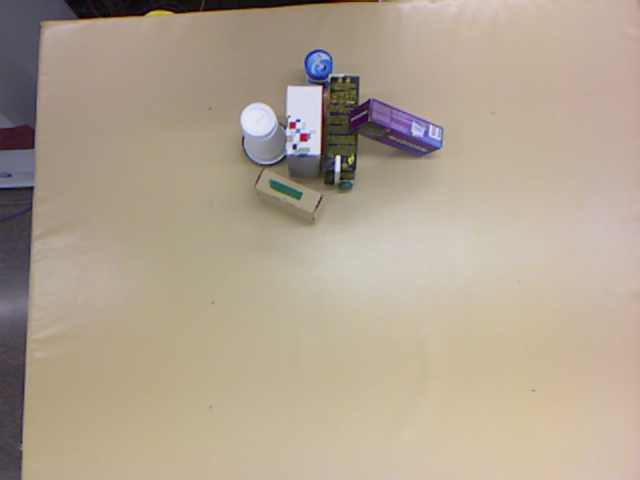
\includegraphics[width=6cm]{Img/experiments/exp1/image.png}
\caption{}
\end{subfigure}
\begin{subfigure}[t]{0.45\textwidth}
\centering
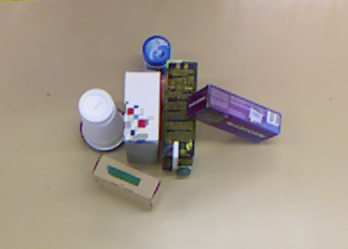
\includegraphics[width=6cm]{Img/experiments/exp1/objects.png}
\caption{}
\end{subfigure}
\caption{}
\end{figure}
We first present the results of a run, next we comment the results of the planning system obtained from 5 runs of this experiment. 


\iffalse
In this chapter the performance of the proposed task planner for the considered task is evaluated by performing several experiments with the aim to study the quality, its benefits and its limitations.

To get the quality of the task planner the strategy defined in the article \citep{Benchmarking} by Amignoni et al. In that article they proposed a general method to evaluated the quality of a task planner. 
First they define a functionality benchmark\footnote{A functionality benchmark is a benchmark of specific robotic task. In the case of this thesis a benchmark of the task planner.} thought 4 elements:
\begin{itemize}
\item Description: a high level, general, description of the functionality
\item Input/Output: the information available to the module implementing the function-
ality when executed, and the expected outcome.
\item Benchmarking data: the data needed to perform the evaluation of the performance
of the functional module.
\item Metrics: algorithms to process benchmarking data in an objective way.
\end{itemize}

Regarding the benchmarking of a task planner those elements are defined as:
\begin{itemize}
\item [\textbf{Description:}] Given a initial state and a goal state find a set of actions to reach the goal.
\item [\textbf{Input/Output:}] The inputs are the PDDL domain and problem descriptions. The output is a plan expressed as sequence of actions.
\item [\textbf{Benchmarking data:}] Some data has to be supplied by the robot, including: the input
given to the planner, the output (i.e., the plan) delivered by the planner, and the
performance data for the planner (e.g., memory and time needed). According to
the planning approach, other data might be required. Other data will be possibly collected when a plan is
actually executed, including: time needed to execute each action and time needed
to execute the whole plan.
\item [\textbf{Metrics:}] Metrics are mainly related to good plan quality and to solving time. The target of benchmarking task planning is twofold: to asses the quality of the
plan produced (e.g., in terms of the cost for executing it and its likelihood to succeed) and to assess the quality of the
planning process (i.e., how fast is the plan generated and how much resources are needed to do so). Possible metrics are:
\begin{itemize}
\item \textsl{Levenshtein distance}\footnote{\href{https://en.wikipedia.org/wiki/Levenshtein_distance} {https://en.wikipedia.org/wiki/Levenshtein\_distance}} is a metric that specifies the distance between two strings, in this case a plan can be though as a sequence of character, where each action with a determined object of interest is a character of the string. The Levenshtein distance between the two lists is calculated to measure the quality of the plan. Levenshtein distance
$L_{A,B}(|A|,|B|)$ between two lists A and B is calculated as
\begin{align*}
L_{A,B}(i,j) &= \max(i,j) \qquad if \quad \min(i,j)=0 \\
L_{A,B}(i,j) &= \min(L_{A,B}(i-1,j)+1, \\
& \qquad \quad L_{A,B}(i,j-1)+1,
\\ & \qquad \quad L_{A,B}(i-1,j-1)+1_{a_i \neq b_i})
\qquad otherwise
\end{align*}
where $|A|$ is the length of plan A, and $1_{a_i \neq b_i}$ is equal to 0 if the action $a_i$ is the same of action $b_i$. This metric will be used to evaluate the distance between the optimal plan returned by the planner in the first frame and the real executed plan. 
\item Number of actions correctly performed in the correct order (e.g., number of
objects delivered to their correct destination). 
\item Time required to construct a plan and time to perform it. 
\end{itemize}
\end{itemize}
We will also evaluate the difference of executing the initial plan and executing the plan with the replanning technique in terms of time and number of correct actions. As well also the number of bad, or dangerous, object manipulations due to the lack of replanning, lack of probability and geometric constraints in the planner . 

It is important highlighting that what has been done is not a benchmarking since no comparison is done with other state of the art planners, but the commented guideline for benchmarks has been used in order to get some useful metrics in order to assert the quality of the planner. 

Kinds of possible experiment to do:
\begin{itemize}
\item show experiments first trying only separating the object (infinite loop behaviour) and then coupling the grasping action. 
\item Show the results of the planner with the pushing length chosen not accordingly to the surrounding objects but accordingly to the pushed one. From that comment the improvements.
\item Show normal experiment where everything works
\item Show situation why we are going to consider the risk as cost in the action. 
\end{itemize}

Metrics to considers:
\begin{itemize}
\item number of objects
\item segmentation time
\item Total solution time
\item planning time
\item total solution
\item Inverse kinematics solution time (this will probably used to justify the backtracking method)
\item Predicates time computation (maybe add collision checking time in )
\end{itemize}


Find a way to get the computational complexity. 

\begin{figure}
\centering
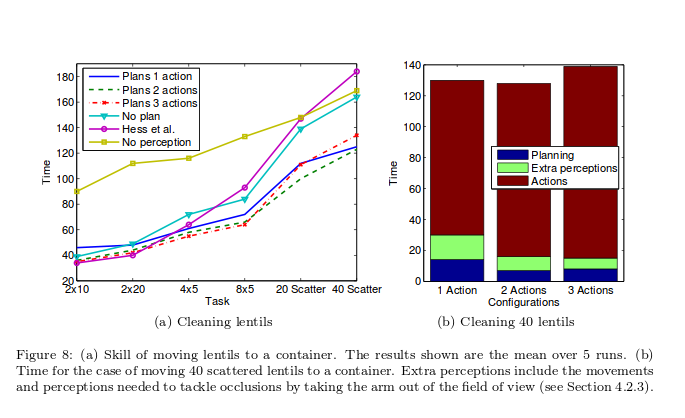
\includegraphics[width=\textwidth]{Img/general/experiments.png}
\end{figure}

\begin{itemize}
\item 2 experiments in which everything works
\item experiment which shows the limitaiton of the planner
\end{itemize}

\fi